\documentclass[aspectratio=43]{beamer}
% \documentclass[aspectratio=169]{beamer}

% Title --------------------------------------------
\title[Lecture 3: Causality]{\Large Causality}
\author[]{Francisco Villamil}
\date[]{Research Design for Social Sciences\\MA Computational Social Science, UC3M\\Fall 2023}

%%% NOTE -- CHECK THIS: https://github.com/paulgp/beamer-tips


%%% Building heavily on https://github.com/kylebutts/templates

% xcolor, define them
\usepackage{xcolor}

% TEXT COLORS
\definecolor{red}{HTML}{9a2515}
\definecolor{yellow}{HTML}{EBC944}
\definecolor{asher}{HTML}{555F61}
\definecolor{jet}{HTML}{131516}

% THEME COLORS
\definecolor{accent}{HTML}{107895}
\definecolor{accent2}{HTML}{9a2515}

% Color commands
\newcommand\red[1]{{\color{red}#1}}
\newcommand\yellow[1]{{\color{yellow}#1}}
\newcommand\asher[1]{{\color{asher}#1}}

\newcommand\BGred[1]{{\colorbox{red!80!white}{#1}}}
\newcommand\BGyellow[1]{{\colorbox{yellow!80!white}{#1}}}
\newcommand\BGasher[1]{{\colorbox{asher!80!white}{#1}}}

% Appendix numbering
\usepackage{appendixnumberbeamer}

% Beamer Options -------------------------------------

% Background
\setbeamercolor{background canvas}{bg = white}

% Change text margins
\setbeamersize{text margin left = 25pt, text margin right = 15pt}

% \alert
\setbeamercolor{alerted text}{fg = accent2}

% Frame title
\setbeamercolor{frametitle}{bg = white, fg = jet}
\setbeamercolor{framesubtitle}{bg = white, fg = accent}
\setbeamerfont{framesubtitle}{size = \small, shape = \itshape}

% Block
\setbeamercolor{block title}{fg = white, bg = accent2}
\setbeamercolor{block body}{fg = jet, bg = jet!10!white}

% Title page
\setbeamercolor{title}{fg = jet}
\setbeamercolor{subtitle}{fg = accent}

%% Custom \maketitle and \titlepage
\setbeamertemplate{title page}
{
    \begin{centering}
      % \vspace{20mm}
      {\Large \usebeamerfont{title}\usebeamercolor[fg]{title}\inserttitle}\\ \vskip0.25em%
      \ifx\insertsubtitle\@empty%
      \else%
        {\usebeamerfont{subtitle}\usebeamercolor[fg]{subtitle}\insertsubtitle\par}%
      \fi%
      {\vspace{10mm}\insertauthor}\\
      \ifx\insertinstitute\@empty%
      \else%
        {\vspace{5mm}\color{asher}\scriptsize{\insertinstitute}}\\\vspace{5mm}
      \fi%
      {\color{asher}\small{\insertdate}}\\
    \end{centering}
}

% Table of Contents
\setbeamercolor{section in toc}{fg = accent!70!jet}
\setbeamercolor{subsection in toc}{fg = jet}

% Button
\setbeamercolor{button}{bg = accent}

% Remove navigation symbols
\setbeamertemplate{navigation symbols}{}

% Table and Figure captions
\setbeamercolor{caption}{fg=jet!70!white}
\setbeamercolor{caption name}{fg=jet}
\setbeamerfont{caption name}{shape = \itshape}

% Put slide number / total slides at the bottom right
\makeatother
\makeatletter
\setbeamertemplate{footline} %{\hfill\insertframenumber/\inserttotalframenumber}
{%
  \leavevmode%
  \hbox{
  \begin{beamercolorbox}[wd=\paperwidth,ht=2.5ex,dp=1.125ex,leftskip=.3cm,rightskip=.3cm plus1fil]{footlinecolor}%
    \color{asher}{{\let\hyperlink\@secondoftwo\insertshorttitle}\hfill\insertshortauthor\hfill\insertshortdate\hfill\insertframenumber/\inserttotalframenumber}
  \end{beamercolorbox}}%
  \vskip0pt%
}
\makeatother
\makeatletter

% Bullet points

%% Fix left-margins
\settowidth{\leftmargini}{\usebeamertemplate{itemize item}}
\addtolength{\leftmargini}{\labelsep}

%% enumerate item color
\setbeamercolor{enumerate item}{fg = accent}
\setbeamerfont{enumerate item}{size = \small}
\setbeamertemplate{enumerate item}{\insertenumlabel.}

%% itemize
\setbeamercolor{itemize item}{fg = accent!70!white}
\setbeamerfont{itemize item}{size = \small}
\setbeamertemplate{itemize item}[circle]
\setlength{\itemsep}{0pt plus 6pt}

%% right arrow for subitems
\setbeamercolor{itemize subitem}{fg = accent!60!white}
\setbeamerfont{itemize subitem}{size = \small}
\setbeamertemplate{itemize subitem}{$\rightarrow$}

\setbeamertemplate{itemize subsubitem}[square]
\setbeamercolor{itemize subsubitem}{fg = jet}
\setbeamerfont{itemize subsubitem}{size = \small}

% References

%% Bibliography Font, roughly matching aea
\setbeamerfont{bibliography item}{size = \footnotesize}
\setbeamerfont{bibliography entry author}{size = \footnotesize, series = \bfseries}
\setbeamerfont{bibliography entry title}{size = \footnotesize}
\setbeamerfont{bibliography entry location}{size = \footnotesize, shape = \itshape}
\setbeamerfont{bibliography entry note}{size = \footnotesize}

\setbeamercolor{bibliography item}{fg = jet}
\setbeamercolor{bibliography entry author}{fg = accent!60!jet}
\setbeamercolor{bibliography entry title}{fg = jet}
\setbeamercolor{bibliography entry location}{fg = jet}
\setbeamercolor{bibliography entry note}{fg = jet}

%% Remove bibliography symbol in slides
\setbeamertemplate{bibliography item}{}





% Links ----------------------------------------------

\usepackage{hyperref}
\hypersetup{
  colorlinks = true,
  linkcolor = accent2,
  filecolor = accent2,
  urlcolor = accent2,
  citecolor = accent2,
}


% Line spacing --------------------------------------
\usepackage{setspace}
\setstretch{1.2}


% \begin{columns} -----------------------------------
\usepackage{multicol}


% % Fonts ---------------------------------------------
% % Beamer Option to use custom fonts
% \usefonttheme{professionalfonts}
%
% % \usepackage[utopia, smallerops, varg]{newtxmath}
% % \usepackage{utopia}
% \usepackage[sfdefault,light]{roboto}
%
% % Small adjustments to text kerning
% \usepackage{microtype}



% Remove annoying over-full box warnings -----------
\vfuzz2pt
\hfuzz2pt


% Table of Contents with Sections
\setbeamerfont{myTOC}{series=\bfseries, size=\Large}
\AtBeginSection[]{
        \frame{
            \frametitle{Roadmap}
            \tableofcontents[current]
        }
    }


% References ----------------------------------------
\usepackage[
    citestyle= authoryear,
    style = authoryear,
    natbib = true,
    backend = biber
]{biblatex}

% Smaller font-size for references
\renewcommand*{\bibfont}{\small}

% Remove "In:"
\renewbibmacro{in:}{}

% Color citations for slides
\newenvironment{citecolor}
    {\footnotesize\begin{color}{accent2}}
    {\end{color}}

\newcommand{\citetcolor}[1]{{\footnotesize\textcolor{asher}{\citet{#1}}}}
\newcommand{\citepcolor}[1]{{\footnotesize\textcolor{asher}{\citep{#1}}}}

% Tables -------------------------------------------
% Tables too big
% \begin{adjustbox}{width = 1.2\textwidth, center}
\usepackage{adjustbox}
\usepackage{array}
\usepackage{threeparttable, booktabs, adjustbox}

% Fix \input with tables
% \input fails when \\ is at end of external .tex file

\makeatletter
\let\input\@@input
\makeatother

% Tables too narrow
% \begin{tabularx}{\linewidth}{cols}
% col-types: X - center, L - left, R -right
% Relative scale: >{\hsize=.8\hsize}X/L/R
\usepackage{tabularx}
\newcolumntype{L}{>{\raggedright\arraybackslash}X}
\newcolumntype{R}{>{\raggedleft\arraybackslash}X}
\newcolumntype{C}{>{\centering\arraybackslash}X}

% Figures

% \imageframe{img_name} -----------------------------
% from https://github.com/mattjetwell/cousteau
\newcommand{\imageframe}[1]{%
    \begin{frame}[plain]
        \begin{tikzpicture}[remember picture, overlay]
            \node[at = (current page.center), xshift = 0cm] (cover) {%
                \includegraphics[keepaspectratio, width=\paperwidth, height=\paperheight]{#1}
            };
        \end{tikzpicture}
    \end{frame}%
}

% subfigures
\usepackage{subfigure}


% Highlight slide -----------------------------------
% \begin{transitionframe} Text \end{transitionframe}
% from paulgp's beamer tips
\newenvironment{transitionframe}{
    \setbeamercolor{background canvas}{bg=accent!60!black}
    \begin{frame}\color{accent!10!white}\LARGE\centering
}{
    \end{frame}
}


% Table Highlighting --------------------------------
% Create top-left and bottom-right markets in tabular cells with a unique matching id and these commands will outline those cells
\usepackage[beamer,customcolors]{hf-tikz}
\usetikzlibrary{calc}
\usetikzlibrary{fit,shapes.misc}

% To set the hypothesis highlighting boxes red.
\newcommand\marktopleft[1]{%
    \tikz[overlay,remember picture]
        \node (marker-#1-a) at (0,1.5ex) {};%
}
\newcommand\markbottomright[1]{%
    \tikz[overlay,remember picture]
        \node (marker-#1-b) at (0,0) {};%
    \tikz[accent!80!jet, ultra thick, overlay, remember picture, inner sep=4pt]
        \node[draw, rectangle, fit=(marker-#1-a.center) (marker-#1-b.center)] {};%
}


\usepackage{tikz}
\usetikzlibrary{graphs}
\usepackage{listings}

\definecolor{codegreen}{rgb}{0,0.6,0}
\definecolor{codegray}{rgb}{0.5,0.5,0.5}
\definecolor{codepurple}{rgb}{0.58,0,0.82}
\definecolor{backcolour}{rgb}{0.95,0.95,0.92}

\lstdefinestyle{mystyle}{
    backgroundcolor=\color{backcolour},
    commentstyle=\color{codegreen},
    % keywordstyle=\color{backcolour},
    numberstyle=\tiny\color{codegray},
    stringstyle=\color{codepurple},
    basicstyle=\ttfamily\footnotesize,
    breakatwhitespace=false,
    breaklines=true,
    captionpos=b,
    keepspaces=true,
    numbers=left,
    numbersep=5pt,
    showspaces=false,
    showstringspaces=false,
    showtabs=false,
    tabsize=2
}

\lstset{style=mystyle}

\begin{document}
% ====================================================

% ----------------------------------------------------
\begin{frame}
  \titlepage
\end{frame}
% ----------------------------------------------------

% % ----------------------------------------------------
% \begin{frame}
% \frametitle{Missing data in DAG framework}
% \centering
%
% Missing completely at random (MCAR)
% Missing at random (MAR)
% Missing not at random (MNAR)
%
% \end{frame}
% % ----------------------------------------------------

\section{Intro to explanation}

% ----------------------------------------------------
\begin{frame}
\frametitle{About prediction}
\centering

\begin{itemize}
  \item<1-> What is prediction?
  \item[]<2->
  \item[]<2-> The two concepts of prediction:
  \item<2-> Predicting another variable
  \item<2-> Predicting the future (or out of sample prediction)
\end{itemize}

\end{frame}
% ----------------------------------------------------

% ----------------------------------------------------
\begin{frame}
\frametitle{About prediction}
\centering


\includegraphics[width = \textwidth]{../img/spotify}

\end{frame}
% ----------------------------------------------------

% ----------------------------------------------------
\begin{frame}
\frametitle{About prediction}
\centering

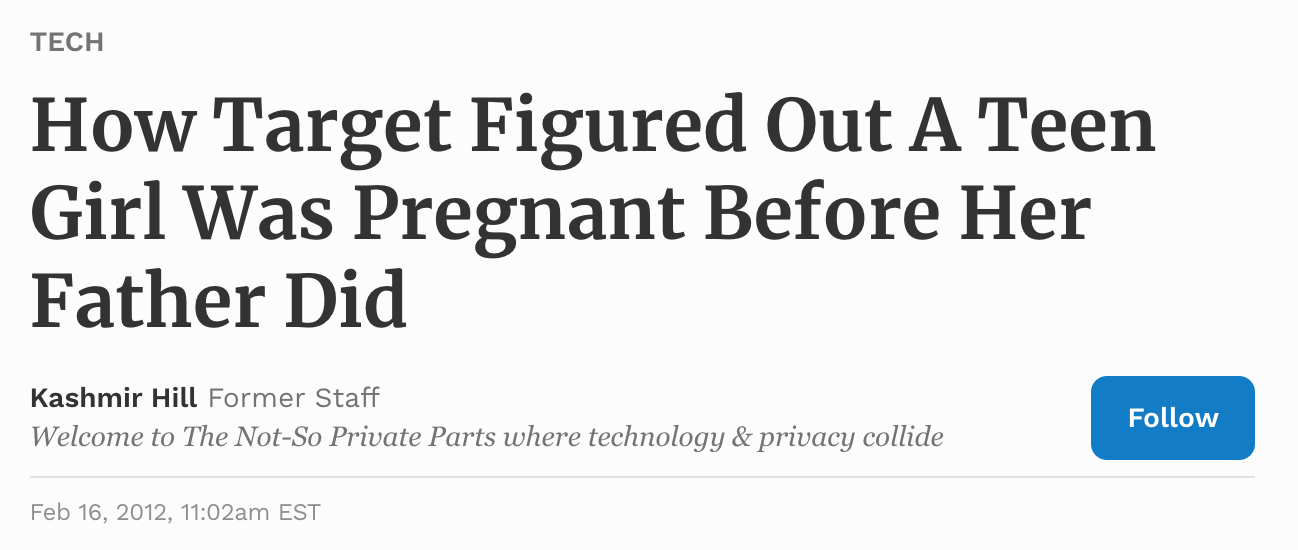
\includegraphics[width = \textwidth]{../img/target_pregnancy}

\end{frame}
% ----------------------------------------------------

% ----------------------------------------------------
\begin{frame}
\frametitle{About prediction}
\centering

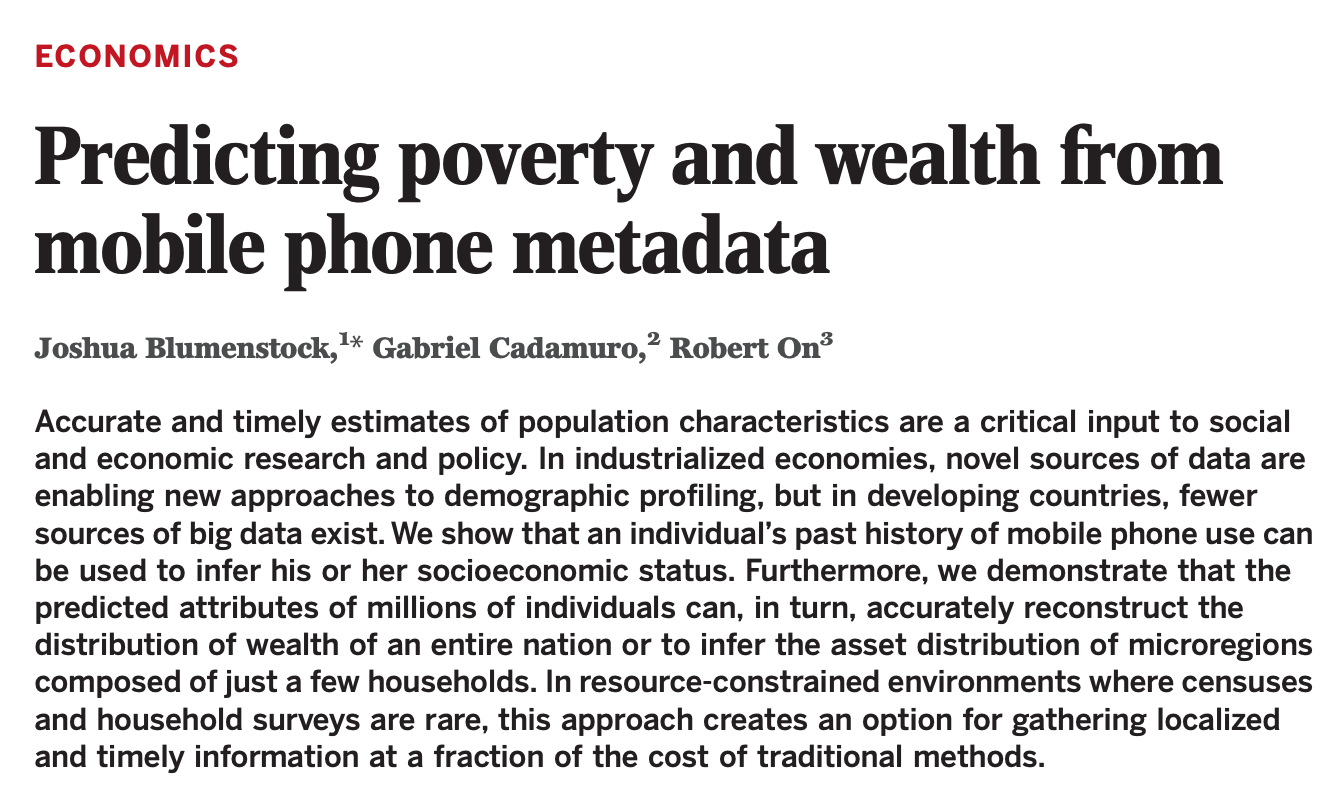
\includegraphics[width = \textwidth]{../img/blumenstock}

\end{frame}
% ----------------------------------------------------

% ----------------------------------------------------
\begin{frame}
\frametitle{About prediction}
\centering

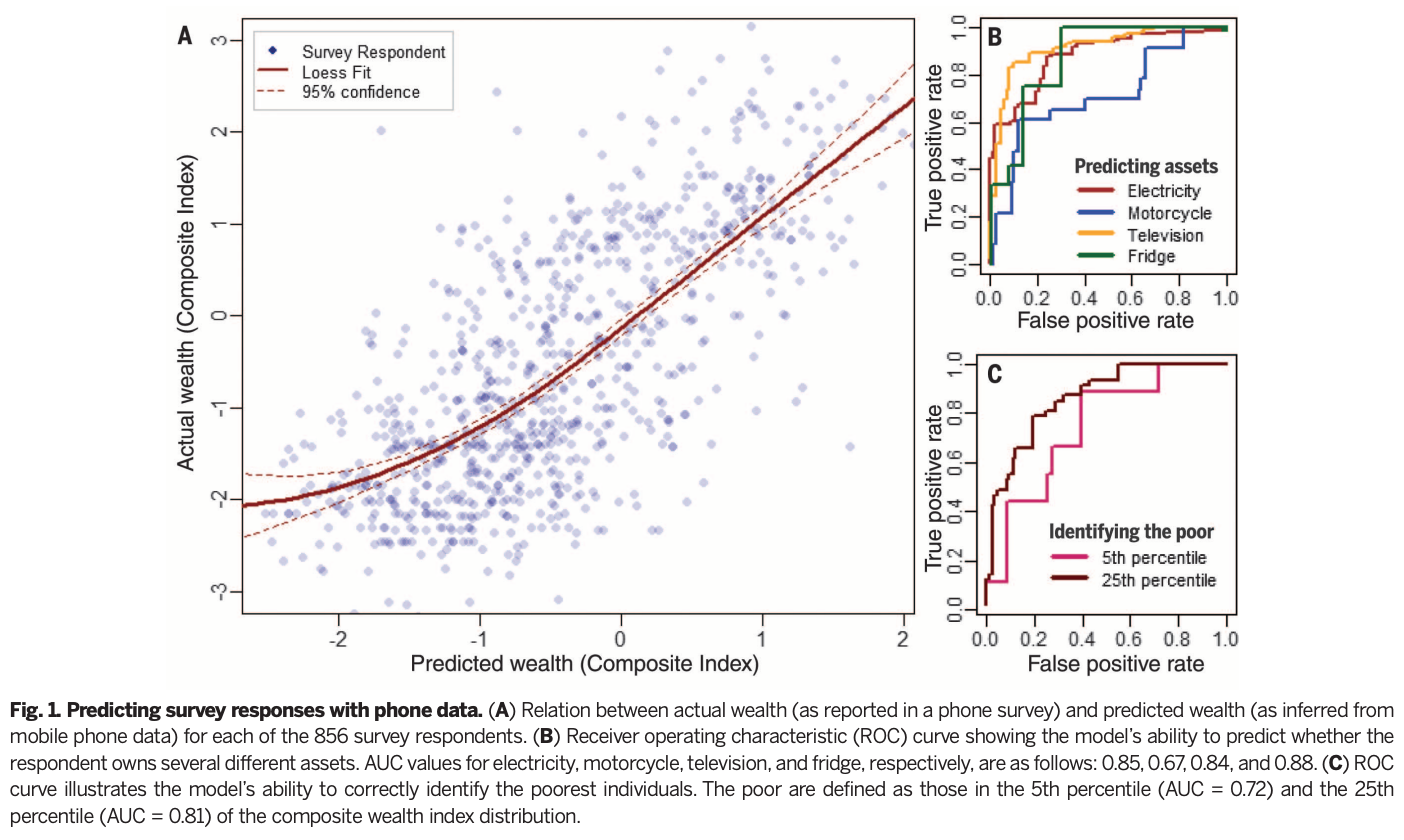
\includegraphics[width = \textwidth]{../img/blumenstock2}

\end{frame}
% ----------------------------------------------------

% ----------------------------------------------------
\begin{frame}
\frametitle{About prediction}
\centering

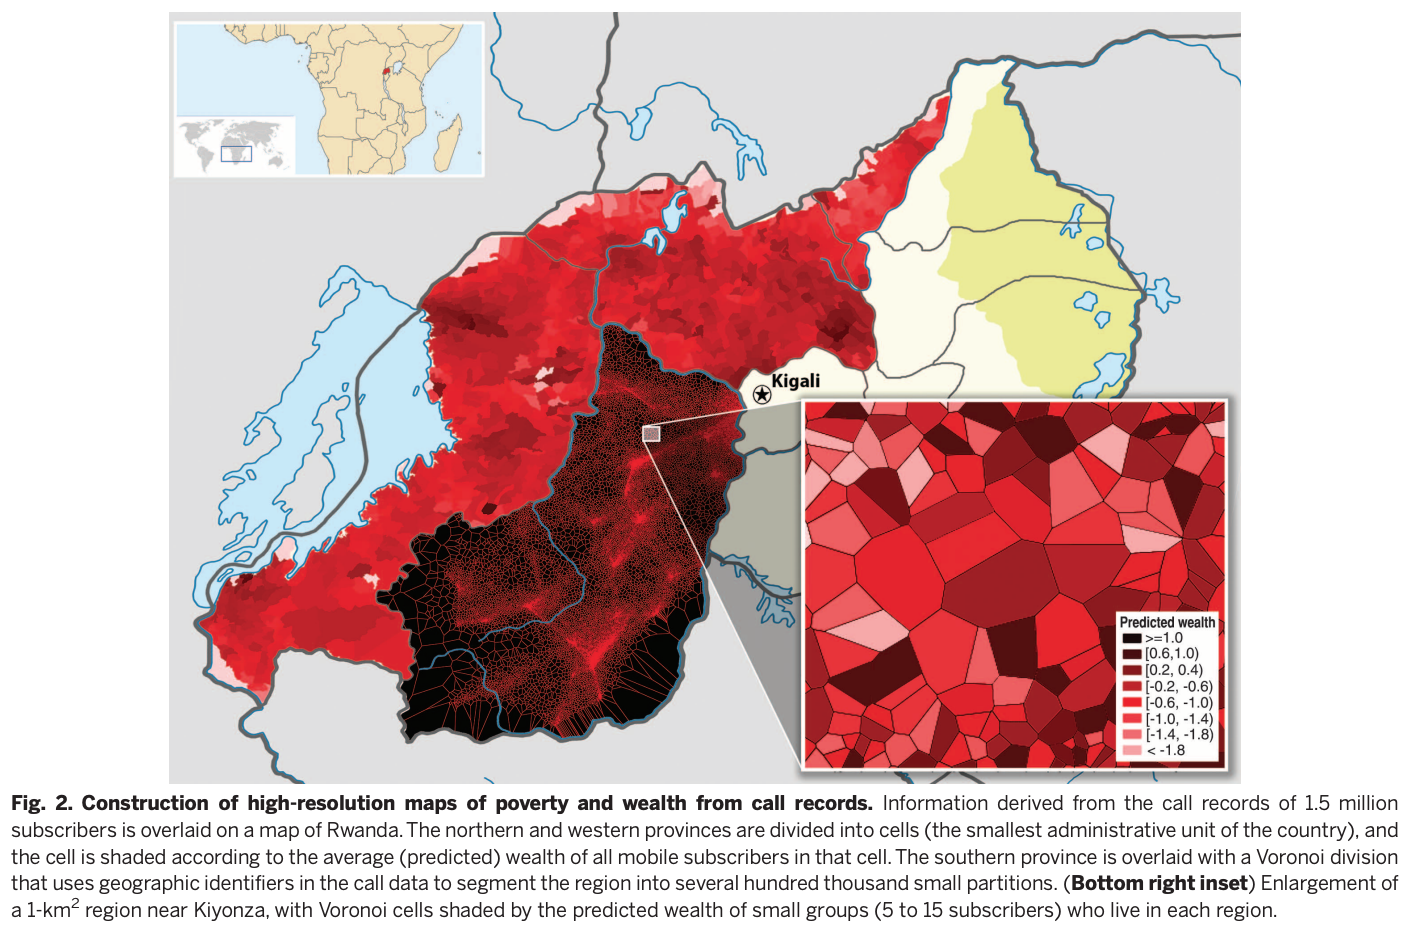
\includegraphics[width = \textwidth]{../img/blumenstock3}

\end{frame}
% ----------------------------------------------------

% ----------------------------------------------------
\begin{frame}
\frametitle{About prediction}
\centering

\begin{itemize}[<+->]
  \item Causality and prediction, is it the same?
  \item The importance of \textbf{counterfactuals} (more on this later)
\end{itemize}

\end{frame}
% ----------------------------------------------------

% ----------------------------------------------------
\begin{frame}
\frametitle{Background: explanatory questions and data}
\centering

\begin{itemize}
  \item When we are dealing with \textit{explanation}, we want to use data to get closer to the \textit{data generating process}
  \item This is the causal process that generates the outcomes that we are measuring (data)
  \item<2-> Example:
  \begin{itemize}
    \item What is the process generating the data that Spotify receives about your music tastes (i.e. song choice)?
    \item<3-> When we try to predict it the way Spotify does, are we using data to uncover the data generating process?
  \end{itemize}
\end{itemize}

\end{frame}
% ----------------------------------------------------

% % ----------------------------------------------------
% \begin{frame}
% \frametitle{Data generating process}
% \centering
%
% \begin{itemize}
%   \item[-] How does the data look like, and what's the data generating process in...
%   \item[]
%   \item Flipping a coin?
%   \item Choosing Mahou instead of another beer brand?
%   \item Going on Erasmus and getting a job?
%   \item[]
%   \item It's kind of like the \textit{causal model} that creates the outcomes, but thinking about data
%   \item When we look for evidence of a causal relationship, we are trying to get closer to the data generating process
% \end{itemize}
%
% \end{frame}
% % ----------------------------------------------------

% % ----------------------------------------------------
% \begin{frame}
% \frametitle{Data generating process}
% \centering
%
% 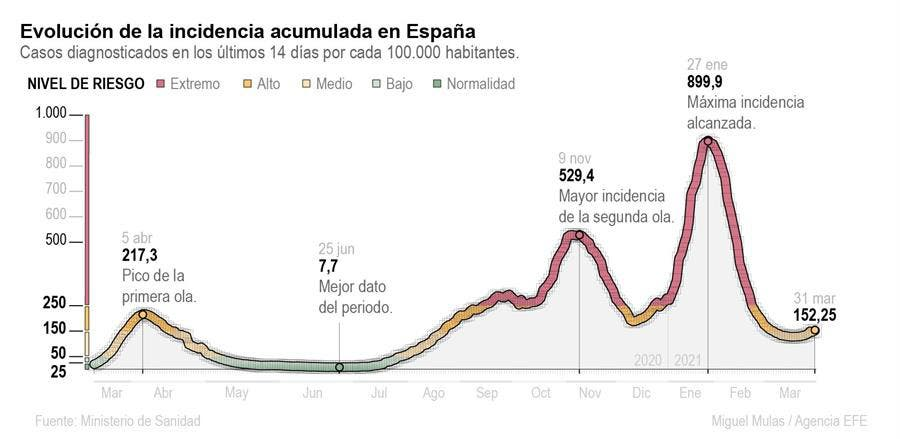
\includegraphics[width = \textwidth]{../img/acumuladaincidencia31marzo}
%
% \begin{itemize}[<+->]
%   \item What the generating process?
%   \item How many variable are involved in generating this outcome?
% \end{itemize}
%
% \end{frame}
% % ----------------------------------------------------
%
% % ----------------------------------------------------
% \begin{frame}
% \frametitle{Thinking about variables and processes/mechanisms}
% \centering
%
% \begin{itemize}
%   \item Think we explain or explain with: variables
%   \item Relationship between them: process
%   \item The main idea is that if we compare different combinations of their values we are going to discover something about the process
% \end{itemize}
%
% \end{frame}
% % ----------------------------------------------------
%
% % ----------------------------------------------------
% \begin{frame}
% \frametitle{Data generating process}
% \centering
%
% 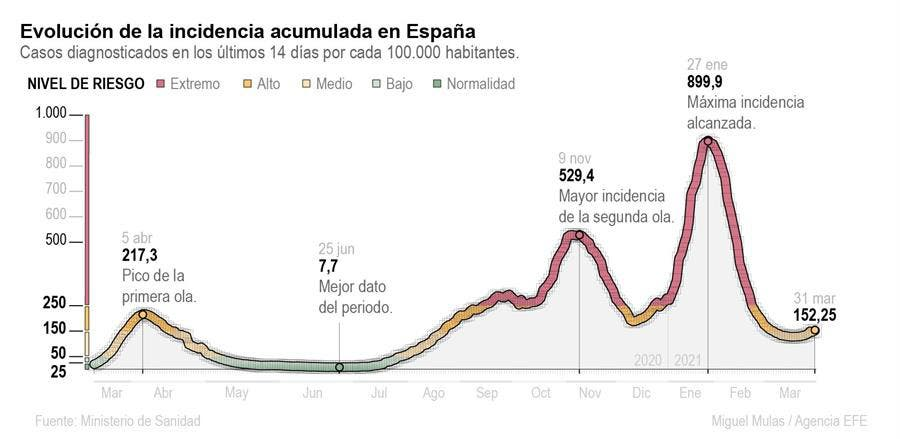
\includegraphics[width = \textwidth]{../img/acumuladaincidencia31marzo}
%
% \begin{itemize}[<+->]
%   \item How could we test different hypotheses? (schools, bars, weather, etc)
% \end{itemize}
%
% \end{frame}
% % ----------------------------------------------------
%
% % ----------------------------------------------------
% \begin{frame}
% \frametitle{DGP and RQs}
% \centering
%
% \begin{itemize}
%   \item Again, we want to state the research question as close as possible to that generating process
%   \item[]
%   \begin{itemize}
%     \item What explains Covid incidence in Madrid?
%     \item What explains Covid incidence in Madrid over time between June 2020 and June 2021
%     \item Do school openings increase Covid incidence in Madrid?
%     \item School openings and Covid incidence evolution in Madrid
%   \end{itemize}
% \end{itemize}
%
% \end{frame}
% % ----------------------------------------------------

% % ----------------------------------------------------
% \begin{frame}
% \frametitle{Example}
% \centering
%
% 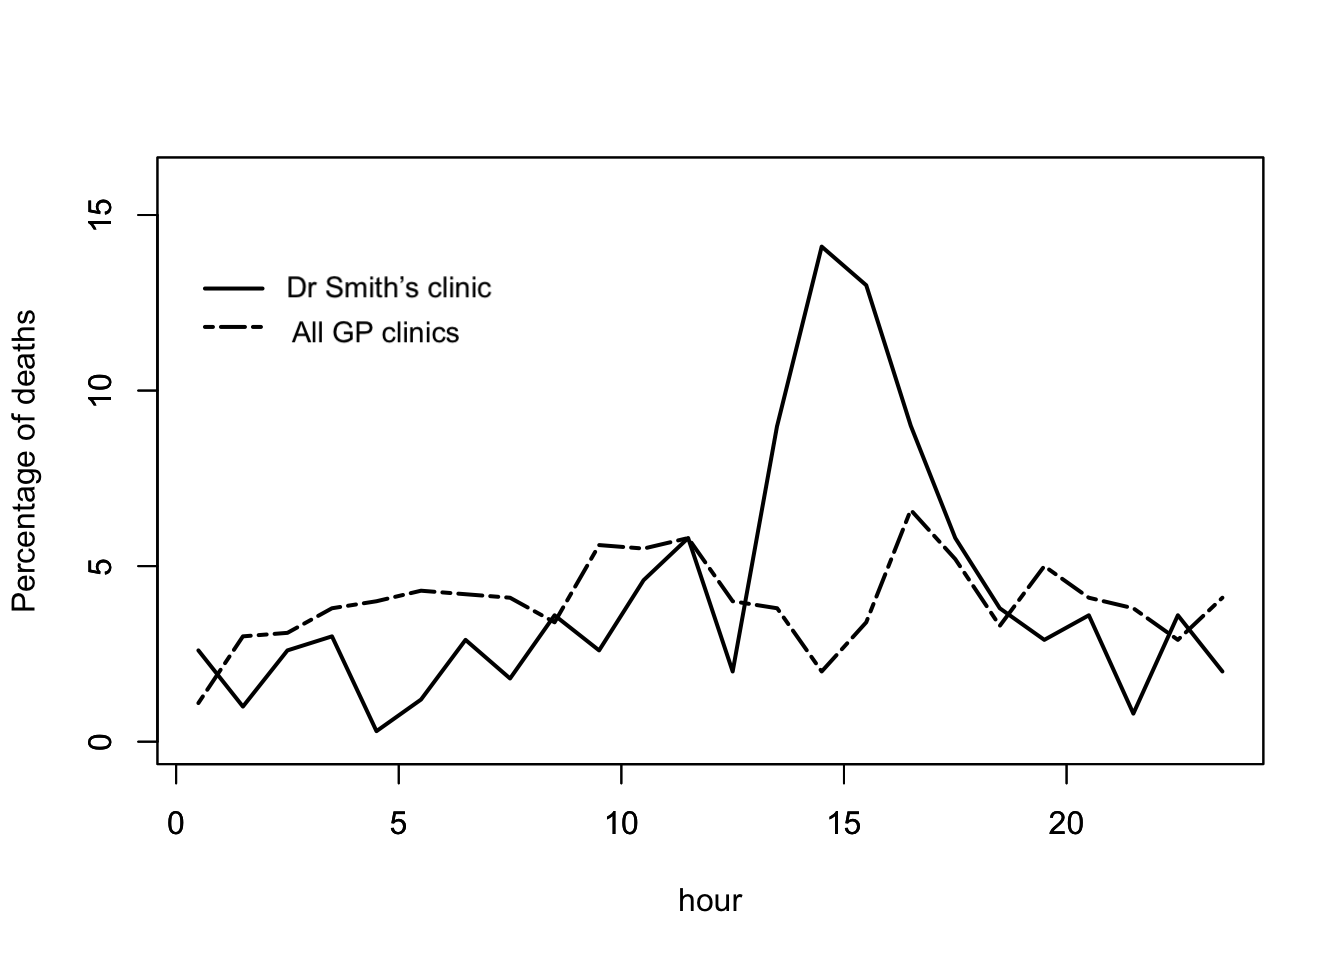
\includegraphics[width = 0.8\textwidth]{../img/shipman}
%
% \begin{itemize}
%   \item Different generating processes? If so, what?
% \end{itemize}
%
% \end{frame}
% % ----------------------------------------------------

\section{Potential outcomes framework}

% ----------------------------------------------------
\begin{frame}
\frametitle{\textit{Explaining} relationships}
\centering

\begin{itemize}[<+->]
  \item Key thing: we want to know whether $X$ actually \textit{causes} $Y$
  \begin{itemize}
    \item I.e., we want to do \textit{causal inference}
  \end{itemize}
  \item (\textbf{Note} that this does not mean that $X$ is the only cause of $Y$, but that \textbf{changing $X$ alters $Y$})
\end{itemize}

\end{frame}
% ----------------------------------------------------

% ----------------------------------------------------
\begin{frame}
\frametitle{\textit{Explaining} relationships}
\centering

\begin{itemize}[<+->]
  \item How could we observe causal relationships? Repeating history
  \item The `fundamental problem of causal inference' is that we cannot
  \begin{itemize}
    \item In other words, that for every unit of observation, we can only observe \textbf{either} $Y(X=0)$ \textbf{or} $Y(X=1)$
  \end{itemize}
  \item If we observe $Y(X=1)$, causal inference essentially means trying to find as good an approximation to $Y(X=0)$ as we can find
  \begin{itemize}
    \item i.e., we want to find something that is valid as a \textit{counterfactual}
  \end{itemize}
\end{itemize}

\end{frame}
% ----------------------------------------------------

% ----------------------------------------------------
\begin{frame}
\frametitle{Potential outcomes framework}
\centering

\begin{itemize}[<+->]
  \item Also called Neyman–Rubin causal model
  \item An effect is the difference between the \textit{actual world} and an \textit{alternative reality} (counterfactual)
  \begin{itemize}
    \item Causal effect of $X$, is $E(Y|X = 1)$ - $E(Y|X = 0)$
  \end{itemize}
\end{itemize}

\end{frame}
% ----------------------------------------------------

% ----------------------------------------------------
\begin{frame}
\frametitle{Potential outcomes framework}
\centering

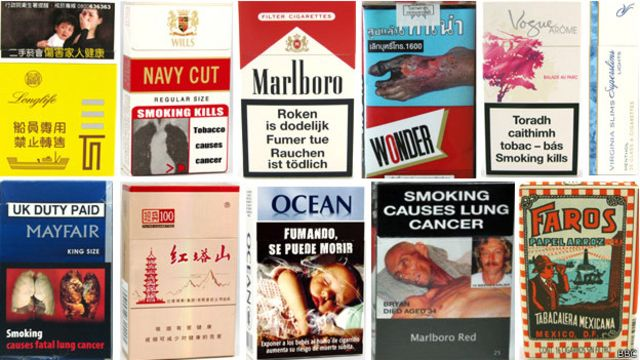
\includegraphics[width = 1\textwidth]{../img/tabaco}

\vspace{10pt}

What is the effect of smoking on life expectancy?

\end{frame}
% ----------------------------------------------------

% ----------------------------------------------------
\begin{frame}
\frametitle{Potential outcomes framework}
\centering

% $E(LExp_{i}|A_{i} = 71, G_{i} = Male, S_{i}=1, E_{i}=0, RM_{i}=1, MC_{i}=1)$

\begin{minipage}{0.7\textwidth}\centering
  \begin{itemize}
    \item<1-> Let's take Gary, a man who smokes, doesn't exercise, but is vegetarian. We can wait and see how long he lives:
    \item<1->[] {\small $E(LExp|S=1, G=Male, E=0, V=1)$}
    \item<2-> The Q is, \textbf{what is the causal effect of smoking} on Gary?
    \item<3-> To know that, we need to estimate the life expectancy of an alternative Gary that is \textit{exactly} the same except for the smoking:
    \item<3->[] {\small $E(LExp|S=0, G=Male, E=0, V=1)$}
    \item<4-> The problem is that the alternative Gary is unobservable: we have a \textbf{missing data problem}
  \end{itemize}
\end{minipage}\hfill
\begin{minipage}{0.3\textwidth}\centering

\includegraphics[width = 0.8\textwidth]{../img/smoking_man}\\Gary
\end{minipage}


\end{frame}
% ----------------------------------------------------


% ----------------------------------------------------
\begin{frame}
\frametitle{Potential outcomes framework}
\centering

\begin{itemize}
  \item<1-> That would be for Gary. What about the `general' effect of smoking?
  \item<2-> Well, we need to find an alternative for every person (smoking and non-smoking), and just calculate the difference between the alternative and the reality:
  \item<2->[] $E[LifeExp_{i}^{1}] - E[LifeExp_{i}^{0}]$
  \item<2->[] which would be the \textbf{Average Treatment Effect} (or \textbf{ATE})
  \item<3-> Problem is we have missing data: we don't have $E[LifeExp_{i}^{1}]$ for non-smokers, and we don't have $E[LifeExp_{i}^{0}]$ for smokers
\end{itemize}

\end{frame}
% ----------------------------------------------------

% ----------------------------------------------------
\begin{frame}
\frametitle{Potential outcomes framework}
\centering

\begin{itemize}
  \item<1-> Same goes with other quantities of interest we'll see:
  \item<2-> \textbf{ATT}, or \textbf{average treatment effect on the treated}:
  \item[]<2-> $E[Y_{i}^{1}|D_{i} = 1] - E[Y_{i}^{0}|D_{i} = 1]$
  \item[]<2-> {\small (effect of smoking among smokers)}
  \item<3-> Or the \textbf{ATC} (or ATU), or \textbf{average treatment effect on the untreated}:
  \item[]<3-> $E[Y_{i}^{1}|D_{i} = 0] - E[Y_{i}^{0}|D_{i} = 0]$
  \item[]<3-> {\small (effect of smoking among non-smokers)}
  \item[]<4->
  \item<4-> When is $ATT \neq ATC$?
\end{itemize}

\end{frame}
% ----------------------------------------------------

\section{Experiments}

% ----------------------------------------------------
\begin{frame}
\frametitle{Estimating causal effects}
\centering

\begin{itemize}
  \item \textbf{So how do we solve this missing data problem?}
  \item[]
  \item<2-> `No causation without manipulation'
  \item<3-> Model initially developed for \textit{experimental data}: randomized controlled trials are the gold-standard in approximating the alternative reality (counterfactual)
\end{itemize}

\end{frame}
% ----------------------------------------------------

% ----------------------------------------------------
\begin{frame}
\frametitle{Issues in experimental designs}
\centering

\begin{itemize}
  \item[] Experiments also have their problems, e.g.:
  \item Non-perfect randomization (esp. if block-r)
  \item SUTVA (or stable unit treatment value assumption)
  \item Attrition
  \item Treatment compliance (estimating the intent-to-treat, or ITT)
  \item External validity
  \item etc
\end{itemize}

\end{frame}
% ----------------------------------------------------

% ----------------------------------------------------
\begin{frame}
\frametitle{Randomization issues}
\centering

\begin{itemize}
  \item Obviously, the basic of any experiment is that \textbf{treatment assignment is random}
  \item It's not frequent, but could happen that this randomization is not well done
  \item Also it might not let us detect the effect, and having statistical issues, especially when using \textit{block} randomization, or \textit{unit} vs. \textit{cluster} randomization
  \item[]
  \item Also could be an issue when doing \textit{block randomization}
\end{itemize}

\end{frame}
% ----------------------------------------------------

% ----------------------------------------------------
\begin{frame}
\frametitle{SUTVA}
\centering

\begin{itemize}
  \item SUTVA stands for \textbf{Stable Unit Treatment Value Assumption}, and it is a key assumption in experimental designs
  \begin{itemize}
    \item It is basically that the outcome in one unit is \textbf{not} affected by treatment assignment in other units
  \end{itemize}
  \item Diffusion effects among subjects?
  \item (This problem is also discussed in causal inference with observational data)
\end{itemize}

\end{frame}
% ----------------------------------------------------

% ----------------------------------------------------
\begin{frame}
\frametitle{Attrition}
\centering

\begin{itemize}
  \item \textbf{Attrition} is just the case when `participants leave the study'
  \item More generally, when some of the units in the experiment do not complete it
  \item The key question is, to what extent is this biasing the results?
\end{itemize}

\end{frame}
% ----------------------------------------------------

% ----------------------------------------------------
\begin{frame}
\frametitle{Treatment compliance}
\centering

\begin{itemize}
  \item Are all units assigned to treatment really exposed to it?
  \item In clinical trials, e.g. do they take the pill or spit it?
  \item How would this look like in an experiment when you pay (treated) individuals to watch TV or use Facebook?
  \item Concept of \textbf{intention-to-treat} (ITT) analyses and the \textbf{complier average causal effect} or \textbf{local average treatment effect} (LATE)
\end{itemize}

\end{frame}
% ----------------------------------------------------

% ----------------------------------------------------
\begin{frame}
\frametitle{External validity}
\centering

\begin{itemize}
  \item To what extend can we \textbf{generalize the results of an experiment}?
  \item This is a more general issue that we will also discuss with observational-data studies, but perhaps very relevant for experiments because of the setting it usually takes place
  \item Example: media exposure studies
  \begin{itemize}
    \item Treatment validity?
    \item Outcome validity of survey hypothetical questions? (behavioral outcomes)
  \end{itemize}
\end{itemize}

\end{frame}
% ----------------------------------------------------

\section{Causal models and diagrams}

% ----------------------------------------------------
\begin{frame}
\frametitle{So how to we approximate $Y^{0}$?}
\centering

\begin{itemize}
  \item Experiments are fine, but often not possible
  \item<2-> How do we do this with \textbf{observational data}?,
    \begin{itemize}
      \item We need to `build' a counterfactual
    \end{itemize}
  \item<3-> Basic idea: we come up with a strategy where the only variation we analyze is (according to us) \textit{due} to the independent variable (cause) we are interested in
  \begin{itemize}
    \item \textbf{Read it again:} it is actually the same idea as in the experimental method, where we use randomization to achieve that
  \end{itemize}
  \item<4-> But in order to do that, we need to be clear about the \textbf{causal model} that is causing $Y$, so we know what we need to control for
  \begin{itemize}
    \item And we're gonna use \BGyellow{causal diagrams} for that
  \end{itemize}
\end{itemize}

\end{frame}
% ----------------------------------------------------


\begin{frame}
\frametitle{Example}
\centering

\begin{itemize}
\item Let's say we want to know whether a cleaner environment makes people happier
\end{itemize}

\end{frame}

\begin{frame}
\frametitle{Example}
\centering

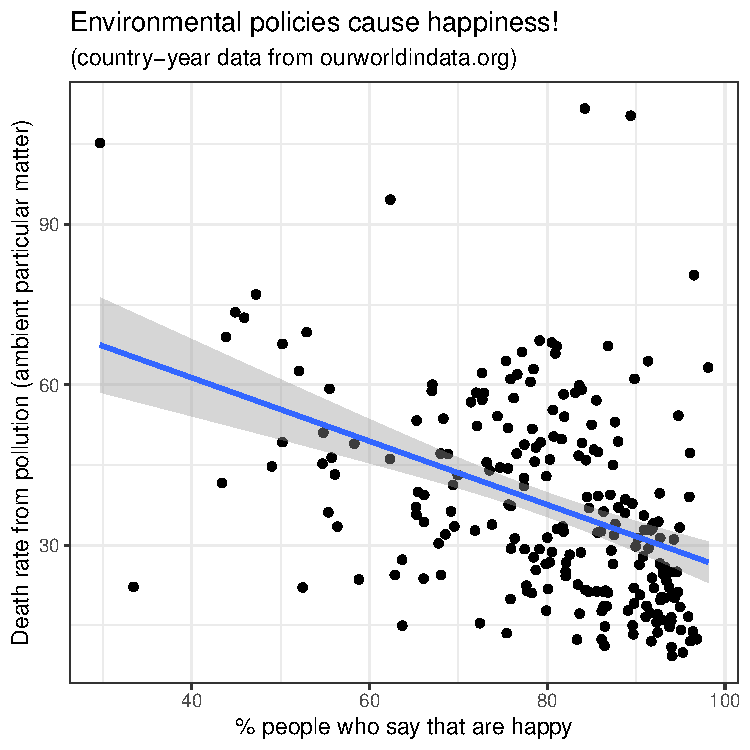
\includegraphics[width = 0.65\textwidth]{../img/happiness_pollution}

\end{frame}

% ----------------------------------------------------
\begin{frame}
\frametitle{Example}
\centering

\begin{itemize}
  \item Remember that out problem (the `fundamental problem of causal inference` etc) is that we can observe e.g. Pakistan, where the level of pollution (measured as death date) is 46, and 58\% of the people say they're happy
  \item But \textbf{we cannot observe} how many people say they are happy in an \textbf{alternative Pakistan} where the pollution death date is 15
  \item So to approximate this, we'll build a causal model to know what we should be controlling for
\end{itemize}

\end{frame}
% ----------------------------------------------------


\begin{frame}
\frametitle{Our causal model}
\centering

\begin{tikzpicture}[every text node part/.style={align=center}, scale = 0.75]

% Process

\node (ep) at (0,0){Cleaner environment};
\node (h) at (7,0){Happiness};
\only<1>{\draw[->] (ep) -- (h);}
\only<1>\node[color=white] (m) at (3.5,3){Wealth};
\only<2->\node (m) at (3.5,3){Wealth};
\only<4>\node (z) at (6,2.75){Z};
\only<2>\draw[->] (m) -- (h);
\only<2-4>\draw[->] (m) -- (ep);
\only<2>{\draw[->, solid] (ep) -- (h);}
\only<3->{\draw[->] (ep) -- (h);}
\only<4>\draw[->] (m) -- (z);
\only<4>\draw[->] (z) -- (h);
\only<5>\draw[->] (m) -- (3.5, 0);

\end{tikzpicture}

\vspace{20pt}

\begin{itemize}
  \only<1>{\item This is our initial causal model: having a cleaner environment makes people happier (because they like looking into a blue sky without smog), and that's it. We do not have to control for anything nor do anything else.}
  \only<2>{\item Wait, but maybe it's about money, isn't it? Actually, wealthier countries tend to have cleaner environments and, at the same time, money causes happiness. \textbf{We need to control for wealth.}}
  \only<3>{\item Or perhaps is not that money increases happiness \textit{per se}, but that it does so through other \textbf{mediators}: wealth allows countries to focus on environment, which increases happiness. \textbf{Again, no need to control.} As long as this is the \textbf{only} mediator.}
  \only<4>{\item We are happy with that model, but we're still missing something. Say we believe that money does not have any direct causal effect, but it does causes some other things (labour conditions, cultural offer, ... let's call them $Z$) and these, in turn, have an effect on happiness. \textbf{We need to control for wealth and all $Z$.}}
  \only<5>{\item (Another thing would be if money \textbf{moderates} the relationship between environmental policies and happiness: spending resources to take care of our environment makes you happier only if you have enough money -- this is an special case, we could talk about heterogenous effects)}
\end{itemize}

\end{frame}

% ----------------------------------------------------
\begin{frame}
\frametitle{Basics of causal inference}
\centering

\begin{itemize}[<+->]
  \item So to come up with an strategy, we need to understand what's going on in terms of the data generating process
  \begin{itemize}
    \item This applies from the most basic strategy (add controls) to the more complicated ones (e.g. evaluating DiD or RDD)
  \end{itemize}
  \item Once we have that, we can \textbf{identify} an effect (in other words: isolating the causal variation from other sources of variation we are not interested in)
\end{itemize}

\end{frame}
% ----------------------------------------------------

% ----------------------------------------------------
\begin{frame}
\frametitle{Causal models, mechanisms, and DAGs}
\centering

\begin{itemize}
  \item We will use \BGyellow{Directed Acyclic Graphs (DAG)} (causal diagrams), a graph where we link \textbf{variables} (nodes) with \textbf{causal effects} (arrows)
  \item[]
  \item[]<2-> A few things:
  \item<3-> Only one-directional causality (\textit{acyclic})
  \begin{itemize}
    \item if you have feedback cycles, write multiple nodes for $t_{1}$, $t_{2}$
  \end{itemize}
  \item<4-> Sometimes: solid lines $\rightarrow$ observed, dashed $\rightarrow$ unobserved ($U$)
  \item<5-> Treatment usually written as $D$ (and $Y$ the outcome)
  \item<6-> Combine variables (usually $B$ for background, or $U$ for unknown)
  \item<7-> No arrow means \textit{no effect}, explicitly
\end{itemize}

\end{frame}
% ----------------------------------------------------

\begin{frame}
\frametitle{This is a DAG}
\centering

\begin{tikzpicture}[every text node part/.style={align=center}, scale = 0.75]

\node (ep) at (0,0){Cleaner environment};
\node (h) at (7,0){Happiness};
\node (z) at (6,2.75){U};
\node (m) at (3.5,3){Wealth};
\draw[->] (m) -- (ep);
\draw[->, dashed] (m) -- (z);
\draw[->, dashed] (z) -- (h);
\draw[->] (ep) -- (h);

\end{tikzpicture}

\end{frame}


% ----------------------------------------------------
\begin{frame}
\frametitle{This is another DAG}
\centering

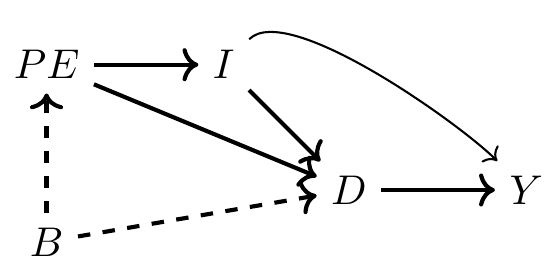
\includegraphics[width = 0.6\textwidth]{../img/dag_earnings}

\vspace{15pt}

\begin{itemize}\footnotesize
  \item Y = earnings (outcome)
  \item D = college education (treatment)
  \item PE = parental education
  \item I = family income
  \item B = unobserved background factors (intelligence, abilities, home, etc)
\end{itemize}



{\tiny from \url{https://mixtape.scunning.com/03-directed_acyclical_graphs}}

\end{frame}
% ----------------------------------------------------

% ----------------------------------------------------
\begin{frame}
\frametitle{Causal models, mechanisms, and DAGs}
\centering

\begin{itemize}
  \item[] We use DAGs for mainly two things related to causal inference:
  \item Drawing up the \textbf{mechanism} that explains the outcome
  \item Come up with the strategy we need to \textbf{identify} the causal effect
  \item[]
  \begin{itemize}
    \item<2-> The difference between the mechanism and the causal model is that not all intermediate steps are relevant for causal inference, even though they do work as an additional check
  \end{itemize}
\end{itemize}

\end{frame}
% ----------------------------------------------------

% ----------------------------------------------------
\begin{frame}
\frametitle{Mediation and moderation}
\centering

\begin{itemize}
\item We usually find more than one variable present in a mechanism
\item Two typical variables: mediator and moderator
\item \BGyellow{Mediation}: a third variable explains the causal relationship between two variables (e.g. flu infection $>$ immune reaction $>$ fever)
\item \BGyellow{Moderation}: a third variable changes the effect of one variable on another (e.g. how age changes the immune reaction)
\end{itemize}

\end{frame}
% ----------------------------------------------------

% ----------------------------------------------------
\begin{frame}
\frametitle{Example: income inequalities}
\centering


\begin{tikzpicture}[every text node part/.style={align=center}, scale = 0.75]

% Process

\node (pe) at (0,0){Parents' education};
\node (i) at (7,0){Income (children)};
\only<1>{\node[color=white] (e) at (5,2.5){Children's education};}
\only<1>{\draw[->] (pe) -- (i);}

\only<2->{\node (e) at (6,2.5){Children's education};}
\only<2>{\draw[->] (pe) -- (e);}
\only<2->{\draw[->] (e) -- (i);}
\only<2->{\draw[->, dashed] (pe) -- (i);}

\only<3->{\node (fi) at (1,2.5){Family income};}
\only<3->{\draw[->] (pe) -- (fi);}
\only<3->{\draw[->] (fi) -- (e);}

\end{tikzpicture}

\vspace{20pt}

\begin{itemize}
  \only<1>{\item Say we want to explain income inequality, and we find that people whose parents went to university earn, on average, more. This would be the basic causal model.}
  \only<2>{\item But \textit{why} it is so? Someone comes and says: ``It's because parents with higher education are more likely to send their children to university and help them get through.''}
  \only<3>{\item And then someone comes and says: ``It's not only that, it's money. Parents with higher education are richer and are able to send their kids to private schools and universities.''}
\end{itemize}

\vspace{20pt}

{\footnotesize (\textit{Note:} in this case I use solid lines for direct effects and dashed lines for indirect effects, kind of)}

\end{frame}
% ----------------------------------------------------

\begin{frame}
\frametitle{DAGs and mechanisms}
\centering

\begin{itemize}[<+->]
\item We can draw the process we're trying to study
\item Main idea: focus on the \textit{data generating process}
  \begin{itemize}
  \item What had to happen for kids with university-degree parents to get richer?
  \item In other words, what mechanisms were in play behind what we see in the data?
  \end{itemize}
\item This matters when choosing our empirical strategy:
  \begin{itemize}
  \item Main identification strategy
  \item Additional checks or implications (testing the mechanism, heterogenous effects, etc)
  \end{itemize}
\end{itemize}

\end{frame}

\section{Back doors and front doors}

% ----------------------------------------------------
\begin{frame}
\frametitle{Front doors and back doors}
\centering

\begin{itemize}
  \item<1-> We are interested in \textit{identifying} the effect of pollution on happiness: that's out \textbf{front door}
  \item<2-> To do so, you have to make sure that the `water flows' through this front door, and not through other `pipe', or back door
  \item[]
  \item<3-> \texttt{Pollution -> Happiness} is our front door
  \item<3-> \texttt{Pollution <- Wealth -> Happiness} is a back door
  \item<4-> How do you close it? Just controlling for \texttt{Wealth}
\end{itemize}

\end{frame}
% ----------------------------------------------------

% ----------------------------------------------------
\begin{frame}
\frametitle{Front doors and back doors}
\centering

\begin{itemize}
  \item There are esentially two ways to do causal inference:
  \item[1.] Close all back doors and leave only the front door open
  \item[] That's where DAGs help to identify these variables
  \item[]
  \item[2.] Using some other method where only the front door is opened
  \item[] (Finding and analysing exogenous variation)
\end{itemize}

\end{frame}
% ----------------------------------------------------

% ----------------------------------------------------
\begin{frame}[fragile]
\frametitle{Off topic: Controlling}
\centering

\begin{itemize}
  \item How does alcohol consumption affect health?
  \item Imagine we take data from a group of people:
\end{itemize}

 \begin{lstlisting}[language=R]
df = data.frame(
  # In this group of people, one-third are rich
  rich = rbinom(500, 1, 0.3)) %>%
  # Rich people have 3x more money to buy whiskey
  mutate(whiskey = 3*rich + runif(500, 0, 4)) %>%
  # Health risk is worse if you drink more whiskey, but rich people have better health overall
  mutate(risk = -2*rich + .3*whiskey + rnorm(500, 2))
 \end{lstlisting}

\end{frame}
% ----------------------------------------------------

% ----------------------------------------------------
\begin{frame}[fragile]
\frametitle{Off topic: Controlling}
\centering

\begin{lstlisting}[language=R]
cor(df$whiskey, df$risk)
[1] -0.1150553
\end{lstlisting}

\end{frame}
% ----------------------------------------------------

% ----------------------------------------------------
\begin{frame}[fragile]
\frametitle{Off topic: Controlling}
\centering

\begin{itemize}
  \item Controlling for \texttt{rich} $\eq$ look at the variation \textbf{not} explained by \texttt{rich}
  \item i.e., take the group prediction out (mean of whiskey/risk for rich or non-rich)
\end{itemize}

\begin{lstlisting}[language=R]
df = df %>%
  group_by(rich) %>%
  mutate(whiskey_resid = whiskey - mean(whiskey),
         risk_resid = risk - mean(risk)) %>%
  ungroup()
\end{lstlisting}

\end{frame}
% ----------------------------------------------------

% ----------------------------------------------------
\begin{frame}[fragile]
\frametitle{Off topic: Controlling}
\centering

\begin{itemize}
  \item The \textit{true} model we created:
  \item[] \texttt{risk = -2 * rich + .3 * whiskey + error}
\end{itemize}

\begin{lstlisting}[language=R]
cor(df$whiskey_resid, df$risk_resid)
[1] 0.3242735
\end{lstlisting}

\end{frame}
% ----------------------------------------------------

% ----------------------------------------------------
\begin{frame}
\frametitle{Front doors and back doors}
\centering

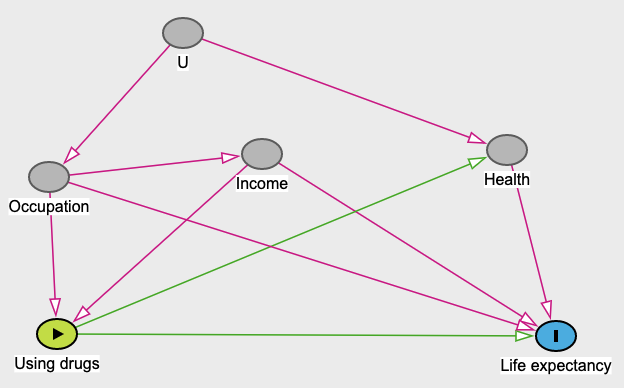
\includegraphics[width = \textwidth]{../img/drugs_dag1}

\end{frame}
% ----------------------------------------------------

% ----------------------------------------------------
\begin{frame}
\frametitle{Front doors and back doors}
\centering

\begin{itemize}
  \item \texttt{Drugs > LifeExp}
  \item \texttt{Drugs > Health > LifeExp}
  \item \texttt{Drugs < Income > LifeExp}
  \item \texttt{Drugs < Occup > LifeExp}
  \item \texttt{Drugs < Occup > Income > LifeExp}
  \item \texttt{Drugs < Occup < U > Income > LifeExp}
  \item \texttt{Drugs < Occup < U > Health > LifeExp}
\end{itemize}

\end{frame}
% ----------------------------------------------------

% ----------------------------------------------------
\begin{frame}
\frametitle{Front doors and back doors}
\centering

\begin{itemize}
  \item {\color{red}{\texttt{Drugs > LifeExp}}}
  \item {\color{red}{\texttt{Drugs > Health > LifeExp}}}
  \item \texttt{Drugs < Income > LifeExp}
  \item \texttt{Drugs < Occup > LifeExp}
  \item \texttt{Drugs < Occup > Income > LifeExp}
  \item \texttt{Drugs < Occup < U > Income > LifeExp}
  \item \texttt{Drugs < Occup < U > Health > LifeExp}
\end{itemize}

\end{frame}
% ----------------------------------------------------

% ----------------------------------------------------
\begin{frame}
\frametitle{Front doors and back doors}
\centering

\begin{itemize}
  \item We just need to control for one of the variables in the path of a back door to close that path
  \item In this example, it would be enough to control for \texttt{income} and \texttt{occupation}
  \item This is the \textbf{back door criterion}
\end{itemize}

\end{frame}
% ----------------------------------------------------


% ----------------------------------------------------
\begin{frame}
\frametitle{Front doors and back doors}
\centering

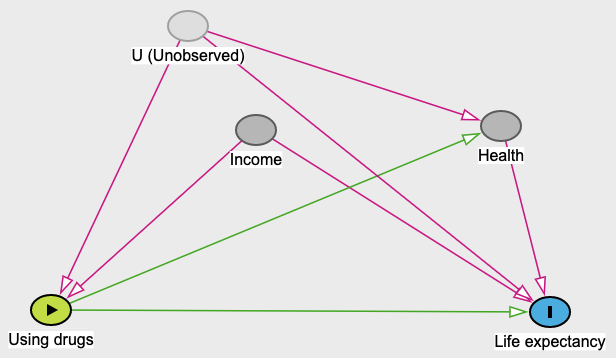
\includegraphics[width = \textwidth]{../img/drugs_dag2}

\end{frame}
% ----------------------------------------------------

% ----------------------------------------------------
\begin{frame}
\frametitle{Front doors and back doors}
\centering

\begin{itemize}
  \item {\color{red}{\texttt{Drugs > LifeExp}}}
  \item {\color{red}{\texttt{Drugs > Health > LifeExp}}}
  \item \texttt{Drugs < Income > LifeExp}
  \item \texttt{Drugs < U > Income > LifeExp}
  \item \texttt{Drugs < U > Health > LifeExp}
  \item \texttt{Drugs < U > LifeExp}
\end{itemize}

\end{frame}
% ----------------------------------------------------

% ----------------------------------------------------
\begin{frame}
\frametitle{Front doors and back doors}
\centering

\begin{itemize}[<+->]
  \item \textbf{What if we control for health?}
  \item We would be blocking part of the causal `water flow' from drugs to life expectancy
  \item That's part of the mechanism: imagine that drugs has a direct effect, e.g. higher probability of dying on an accident, and an indirect effect through its effect on health
  \item (Unless you want to calculate the \textit{direct effect})
  \item[]
  \item So we would have to control for \textbf{U}, which would close all other paths
\end{itemize}

\end{frame}
% ----------------------------------------------------

% ----------------------------------------------------
\begin{frame}
\frametitle{Front doors and back doors}
\centering

\begin{itemize}
  \item {\color{red}{\texttt{Drugs > LifeExp}}}
  \item {\color{red}{\texttt{Drugs > Health > LifeExp}}}
  \item \texttt{Drugs < Income > LifeExp}
  \item \texttt{Drugs < U > Income > LifeExp}
  \item \texttt{Drugs < U > Health > LifeExp}
  \item \texttt{Drugs < U > LifeExp} \textbf{(!)}
  \item[]
  \item Problem? So?
\end{itemize}

\end{frame}
% ----------------------------------------------------

\section{Usual suspects}

% ----------------------------------------------------
\begin{frame}
\frametitle{Usual suspects}
\centering

\begin{itemize}
  \item Confounding
  \item Reverse causality
  \item Bidirectional causation
  \item Selection bias
  \item Collider bias
  \item Post-treatment bias
\end{itemize}


\end{frame}
% ----------------------------------------------------

\begin{frame}
\frametitle{Confounding}
\centering

\begin{itemize}[<+->]
  \item Typical example: as the number of pirates in the oceans decreased, global mean temperature increased. Does it mean the disappearance of pirates is causing global warming?
  \item No, both are caused by the industrial revolution or technological development
  \item Months when people eat more ice-creams, also more people drown in the beach. Ice-creams causing drownings?
\end{itemize}

\end{frame}

\begin{frame}
\frametitle{Reverse causality}
\centering

\begin{itemize}[<+->]
  \item Many examples where correlations we think imply a particular causal effect might be explained by its reverse: Violent videogames making teenagers violence? Maybe violent teeneagers prefer those games. Drug use causes psychological problems? Maybe psychological problems can also cause drug use. (In many cases it's also two-way causality)
  \item ``Hospitals make people sick:'' if you collect data on illness development, you might find that people fare worse if they go to the hospital. Obviously, it's a case of reverse causality: being sick causes going to the hospital.
\end{itemize}

\end{frame}


\begin{frame}
\frametitle{Bidirectional causation}
\centering


\begin{itemize}
  \item (endogenous cycles, $\neq$ reverse causality)
  \item[]
  \item Political values and voting: they way you think makes you vote in a particular way, but the way you vote can also affect the way you think (group influence, cognitive processes, etc)
  \item Can be closely related to selection bias: imagine we go to Madrid Rio and we measure if people doing exercises are more likely to be overweight than those lying around
  \item We probably don't find any result. Does it mean exercise does not decrease overweight? No, it's probably bidirectional causation: overweight makes people more likely to exercise, and exercise reduces overweight
\end{itemize}

\end{frame}

% ----------------------------------------------------
\begin{frame}
\frametitle{}
\centering

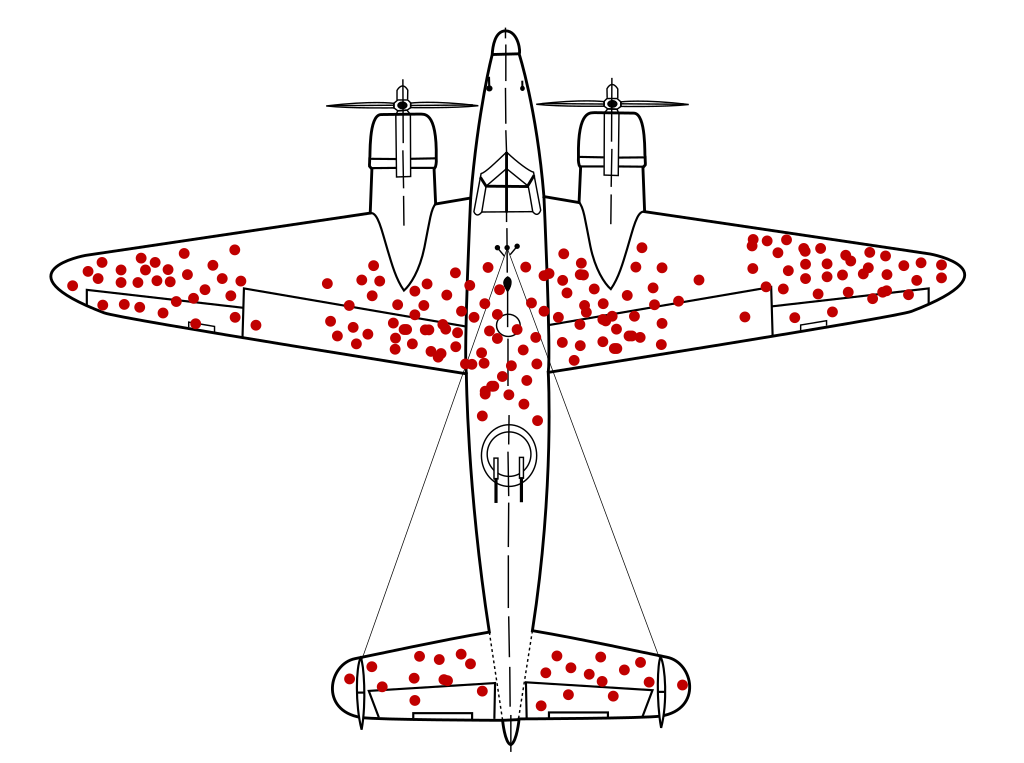
\includegraphics[width = 0.8\textwidth]{../img/Survivorship-bias}

\end{frame}
% ----------------------------------------------------

\begin{frame}
\frametitle{Selection bias}
\centering

\begin{itemize}[<+->]
  \item Our observations are not representative
  \item Famous example from World War II airplanes
  \item Many examples: advice from successful CEOs, ex-heroin addicts more likely to do sports, etc
  \item Why?
  \begin{itemize}
    \item Sampling
    \item Attrition ($\approx$ survivorship bias)
    \item etc
  \end{itemize}
\end{itemize}

\end{frame}


% ----------------------------------------------------
\begin{frame}
\frametitle{Selection bias in causal inference}
\centering

\begin{itemize}
  \item Selection bias in statistics: sampling issue
  \item Quite different in causality: we're dealing with \textbf{selection into treatment}
  \item Remember example from HIV treatments studies
\end{itemize}

\end{frame}
% ----------------------------------------------------

% ----------------------------------------------------
\begin{frame}
\frametitle{Collider bias}
\centering

\begin{tikzpicture}
% nodes %
\node (Y) at (2,0){Outcome};
\node (D) at (-2,0){Treatment};
\node (U) at (0,3){Z};
\draw[->] (D) -- (Y);
\draw[<-] (U) -- (D);
\draw[<-] (U) -- (Y);
\end{tikzpicture}

\end{frame}
% ----------------------------------------------------


% ----------------------------------------------------
\begin{frame}
\frametitle{Collider bias}
\centering


\includegraphics[width = 0.7\textwidth]{../img/crazyhot}

\end{frame}
% ----------------------------------------------------


\begin{frame}[fragile]
\frametitle{Collider bias}
\centering

\begin{itemize}
  \item Are good looking people jerks?
  \item We have 1,000 people, with \textbf{randomly} distributed beauty and niceness
\end{itemize}

 \begin{lstlisting}[language=R]
 df = data.frame(
   niceness = rnorm(1000, mean = 5, sd = 1.5),
   beauty = rnorm(1000, mean = 5, sd = 1.5))
 \end{lstlisting}

\end{frame}

\begin{frame}[fragile]
\frametitle{Collider bias}
\centering

\begin{itemize}
  \item No correlation
\end{itemize}

 \begin{lstlisting}[language=R]
 cor(df$niceness, df$beauty)
 [1] 0.02876464
 \end{lstlisting}

\end{frame}


\begin{frame}
\frametitle{Collider bias}
\centering

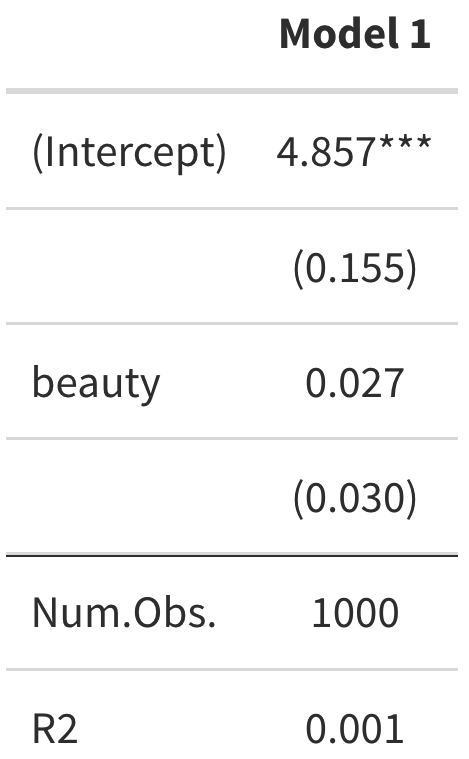
\includegraphics[width = 0.4\textwidth]{../img/collider_m1}

\end{frame}

\begin{frame}
\frametitle{Collider bias}
\centering

\begin{itemize}
  \item Now imagine that we have another variable, the probability of being married, which is we will say is caused by both niceness and beauty:
\end{itemize}

\begin{tikzpicture}
% nodes %
\node (Y) at (2,0){Niceness};
\node (D) at (-2,0){Beauty};
\node (U) at (0,3){Married};
\draw[->] (D) -- (Y);
\draw[<-] (U) -- (D);
\draw[<-] (U) -- (Y);
\end{tikzpicture}

%\begin{lstlisting}[language=R]
%df = df %>%
%  mutate(married = 1.5 * niceness + 3 * beauty) %>%
%  mutate(married = married / max(married))
%\end{lstlisting}

\end{frame}

% ----------------------------------------------------
\begin{frame}
\frametitle{Collider bias}
\centering

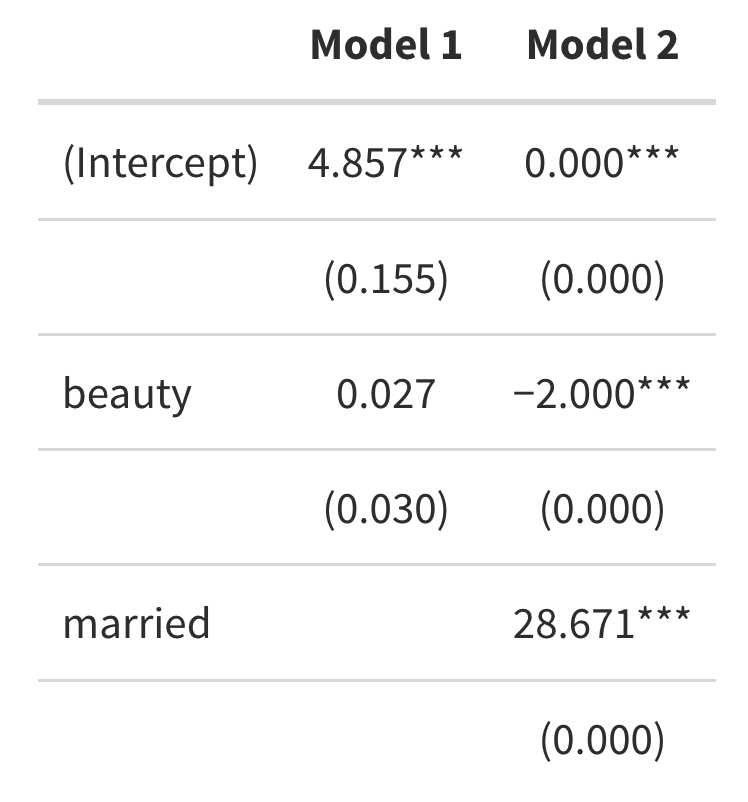
\includegraphics[width = 0.6\textwidth]{../img/collider_m2}

\end{frame}
% ----------------------------------------------------

% ----------------------------------------------------
\begin{frame}
\frametitle{Collider bias}
\centering

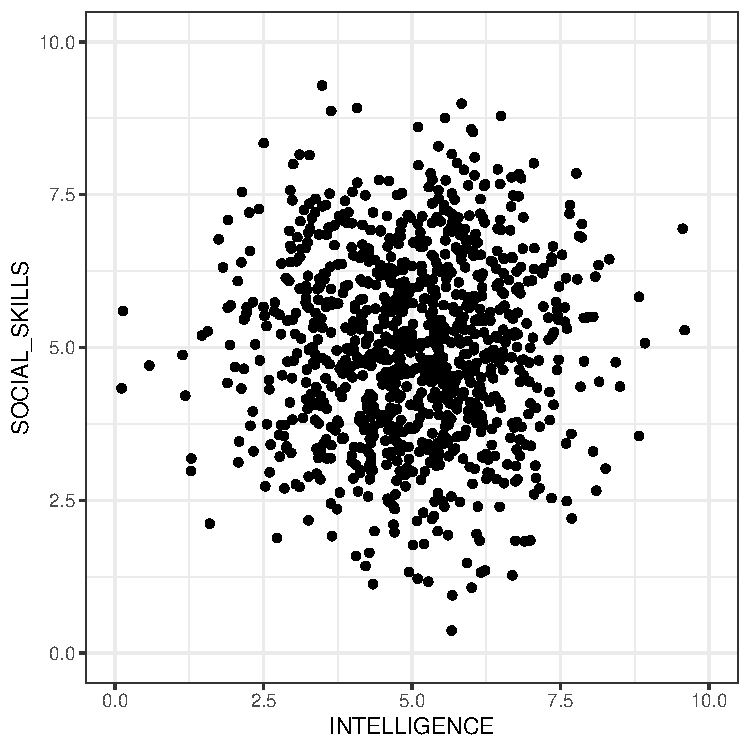
\includegraphics[width = 0.7\textwidth]{../img/collider1}

\end{frame}
% ----------------------------------------------------

% ----------------------------------------------------
\begin{frame}
\frametitle{Collider bias}
\centering

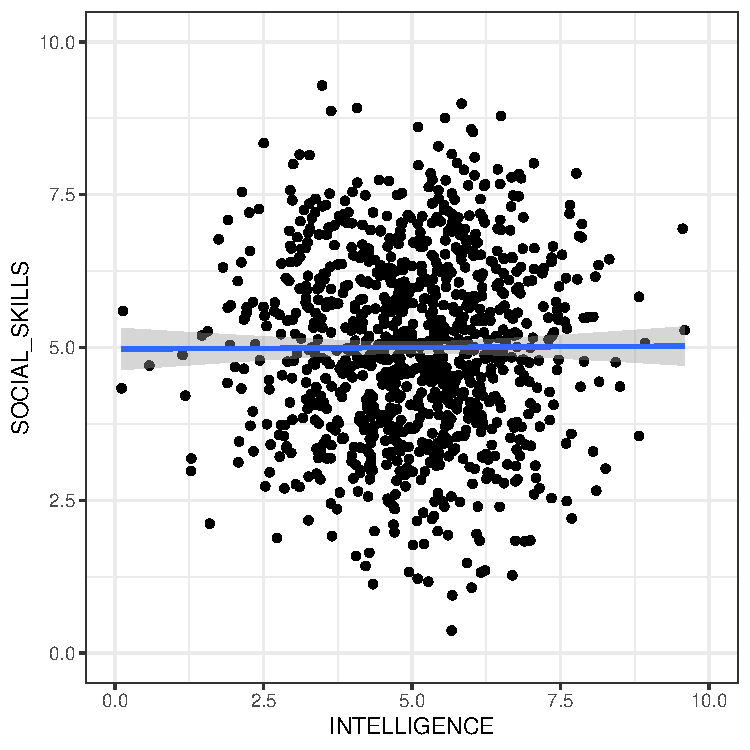
\includegraphics[width = 0.7\textwidth]{../img/collider2}

\end{frame}
% ----------------------------------------------------

% ----------------------------------------------------
\begin{frame}
\frametitle{Collider bias}
\centering

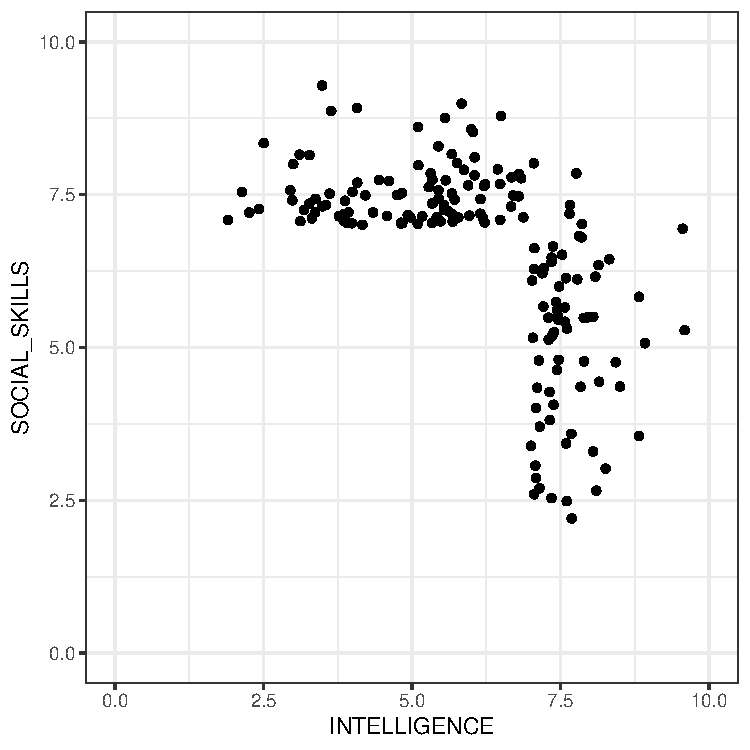
\includegraphics[width = 0.7\textwidth]{../img/collider3}

\end{frame}
% ----------------------------------------------------

% ----------------------------------------------------
\begin{frame}
\frametitle{Collider bias}
\centering

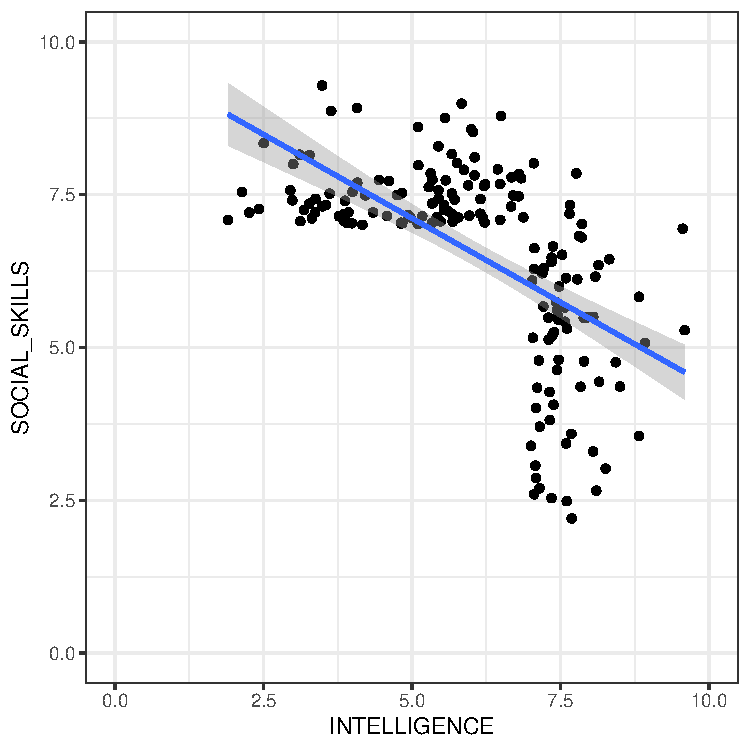
\includegraphics[width = 0.7\textwidth]{../img/collider4}

\end{frame}
% ----------------------------------------------------

% ----------------------------------------------------
\begin{frame}
\frametitle{Collider bias}
\centering

\begin{itemize}
  \item A collider bias \textbf{opens} a path when you control for the variable
\end{itemize}

\end{frame}
% ----------------------------------------------------

% ----------------------------------------------------
\begin{frame}
\frametitle{Collider bias}
\centering

\begin{minipage}{.54\textwidth}\centering
\begin{itemize}
  \item Another example in life sciences where we can only use observational data
  \item Obesity reduces mortality among older people or patients with some chronic diseases (?)
  \item Collider bias? Y = health, X = environment/genetics
\end{itemize}
\end{minipage}\hfill
\begin{minipage}{0.45\textwidth}\centering
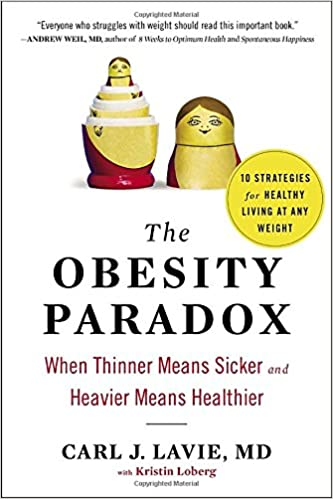
\includegraphics[width = 0.9\textwidth]{../img/obesity_paradox}
\end{minipage}

\end{frame}
% ----------------------------------------------------

% ----------------------------------------------------
\begin{frame}
\frametitle{Collider bias}
\centering

\begin{itemize}
  \item Animated: \url{https://nickchk.com/causalgraphs.html}
\end{itemize}

\end{frame}
% ----------------------------------------------------


% ----------------------------------------------------
\begin{frame}
\frametitle{Post-treatment bias (collider again)}
\centering

\begin{itemize}[<+->]
  \item We want to know whether suffering violence during a civil wars makes people more or less likely to support certain authorities decades after the war
  \item And we say: well, the country develop economically after the war, so maybe it makes sense to control for local increase in GDPpc, because it will also affect support
\end{itemize}

\end{frame}
% ----------------------------------------------------

% ----------------------------------------------------
\begin{frame}
\frametitle{Post-treatment bias (collider again)}
\centering

\begin{tikzpicture}
% nodes %
\node (Y) at (2,0){Support (postwar)};
\node (D) at (-2,0){Violence (war)};
\node (Z) at (0,3){Postwar economic growth};
\draw[->] (D) -- (Y);
\draw[<-] (Z) -- (D);
\draw[->] (Z) -- (Y);
\end{tikzpicture}

\end{frame}
% ----------------------------------------------------

% ----------------------------------------------------
\begin{frame}
\frametitle{Post-treatment bias (collider again)}
\centering

\begin{tikzpicture}
% nodes %
\node (Y) at (2,0){Support (postwar)};
\node (D) at (-2,0){Violence (war)};
\node (Z) at (0,3){Postwar economic growth};
\node (U) at (3,2.5){U};
\draw[->] (D) -- (Y);
\draw[<-] (Z) -- (D);
\draw[->] (Z) -- (Y);
\draw[->, dashed] (U) -- (Z);
\draw[->, dashed] (U) -- (Y);
\end{tikzpicture}

\end{frame}
% ----------------------------------------------------

% ----------------------------------------------------
\begin{frame}
\frametitle{Recap: what should not be controlled for}
\centering

\begin{itemize}
  \item[1.] Front-door paths
  \begin{itemize}
    \item Blocking some of the effect through a mediator variable
    \item (There are almost always mediator variables, so you could potentially just eliminate all the effect you're trying to identify)
  \end{itemize}
  \item[]
  \item[2.] Collider bias
  \begin{itemize}
    \item Opens a new, uncontrolled-for path
    \item Sometimes you might be inadvertently controlling for a collider because of \textit{selection} issues
    \item Extra care with post-treatment bias
  \end{itemize}
\end{itemize}

\end{frame}
% ----------------------------------------------------


%\appendix
%\renewcommand{\theframenumber}{A\arabic{framenumber}}
%\renewcommand{\insertframenumber}{A\arabic{framenumber}}

% ====================================================
\end{document}
